\begin{figure}[h!]
    \centering
    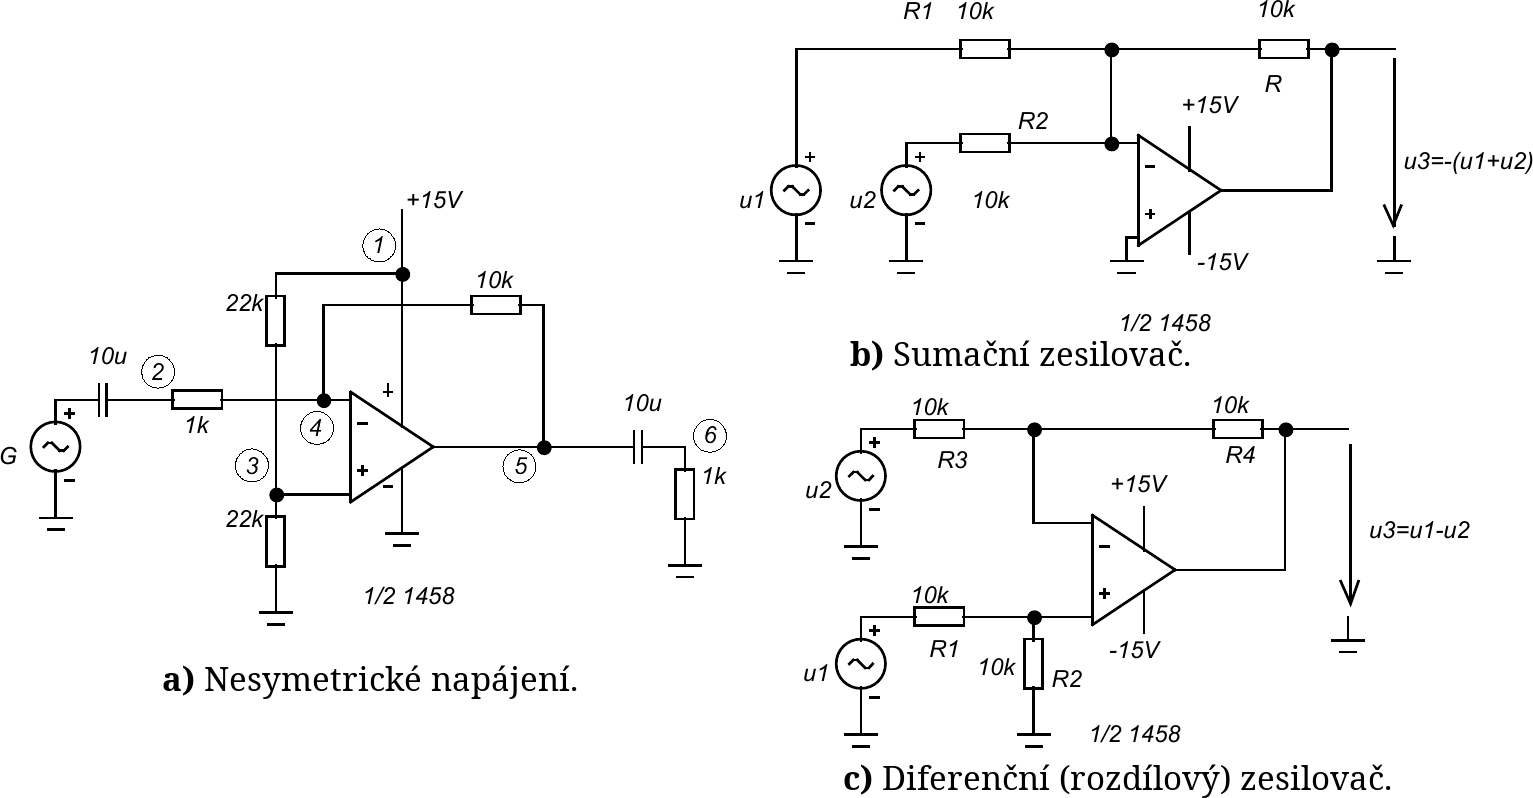
\includegraphics[width=\textwidth]{schema.png}
    \centering
    \caption{Schémata zapojení.}
    \label{fig:schema}
\end{figure}



\subsection{Napájení OZ}

    Rozlišujeme dva základní typy napájení OZ, symetrické a nesymetrické. Sympetrické napětí očekává kladné a záporné napětí na svorkách OZ a potenciál společné země je vůči nim uprostřed, tedy v nule. K tomuto je zapotřebí využít dva zdroje, což je v praxi obtížné, následné zapojení je ale jednodušší. V případě symetrického napájení je na záporné svorce potenciál společné země, stačí nám tedy jeden zdroj. Pokud ale chceme mít jistotu, že výstupní signál nebude zkreslený, je potřeba toto kompenzovat upravením obvodu na vstupu OZ, viz Obr.~\ref{fig:schema}a).


\subsection{Vypočtené hodnoty pro úlohu č. 1}
    \subsubsection{Stejnosměrné poměry v obvodu}
        $ U_1=\qty{15}{\volt} $, $ U_2=\qty{7.5}{\volt} $, $ U_3=\qty{7.5}{\volt} $, $ U_4=\qty{7.5}{\volt} $, $ U_5=\qty{7.5}{\volt} $, $ U_6=\qty{0}{\volt} $, $ U_7=\qty{0}{\volt} $


    \subsubsection{Střídavé poměry v obvodu, pro amplitudu generátru $ U_M=\qty{1}{\volt} $ }
        $ u_1=\qty{0}{\volt} $, 
        $ u_2=\qty{1}{\volt} $, 
        $ u_3=\qty{0}{\volt} $, 
        $ u_4=\qty{0}{\volt} $, 
        $ u_5=\qty{-10}{\volt} $, 
        $ u_6=\qty{-10}{\volt} $\\
        $ A_u=\frac{u_{out}}{u_{in}}=\frac{-10}{1}=-10 $

\subsection{Odvození vztahů pro úlohu č. 2 a 3}
    \subsubsection{Sumační zesilovač, Obr.~\ref{fig:schema}b)}
        $ u_1 $, $ u_2 $, $ u_3 $ \dots Napětí na rezistorech orientovaná stejně jako proudy. 

        $$ u_{out} = -u_3 = -i_3R_3 = -(i_1+i_2)R_3 = -(\frac{u_1}{R_1}+\frac{u_2}{R_2})R_3 $$
        Hodnoty rezistorů jsou stejné, takže platí:
        $$ u_{out} = -(u_1+u_2) $$

    \subsubsection{Diferenční zesilovač, Obr.~\ref{fig:schema}c)}
        $ u_3 $, $ u_4 $ \dots Napětí na rezistorech orientovaná stejně jako proudy. 

        $$ u_{out} = u_2-u_3-u_4 =u_2 -(u_2-u_1\frac{R_2}{R_1+R_2})-R_4i_4 =  u_1\frac{R_2}{R_1+R_2}-\frac{R_4}{R_3}(u_2-u_1\frac{R_2}{R_1+R_2}) $$
        $$ u_{out}= 2u_1\frac{R_2}{R_1+R_2} -u_2\frac{R_4}{R_3}$$
        Hodnoty rezistorů jsou stejné, takže platí:
        $$ u_{out}=u_1-u_2$$

